%======================================%
%-->    Lab: Diodes and Transistors <--%
%--> Author: Charles Edward Pax     <--%
%-->   Date: 2006.02.14             <--%
%======================================%
% NOTE: The README file contains much more detailed descriptions of all the commands you might need.
%
%
\documentclass[11pt,onecolumn]{article}
% This sets the document type to be used to "article" and activates any desired style optioins.
% Options
% ====================
% Name		Description
% --------	-----------
% 10pt		Set font size to 10 points
% 11pt		Set font size to 11 points
% 12pt		Set font size to 12 points
% onecolumn	Set number of columns to one
% twocolumn	Set number of columns to two

\usepackage{color,graphics}
% Options
% ====================
% Name		Description
% --------	-----------
% color		Allows the inclusion of colors.
% graphics	Allows the inclusion of various graphics.
% pstricks	Allows many complex graphic functions such as circuit diagrams.

\begin{document}
% This command tells LaTeX to process the following commands as part of the document body.

\title{Diodes and Transistors}
% This command defines the title of the report for use in the "\maketitle" command below.

\date{February 17, 2006}
% This command defines the date for use in the "\maketitle" command below. You may manually type any date or use one of the following options.
% Options
% ====================
% Name		Description
% --------	-----------
% \today	Includes the date the documents is compiled

\author{Charles Edward Pax}
% This command defines the author's name for use in the "\maketitle" command below.

\maketitle
% This command includes the title, author name, and date in the final document.

%=====================%
%--> Sec: Abstract <--%
%=====================%
\abstract{Demonstrates knowledge of two rectirier circuits and two simple transistor circuits.}
% This command tells LaTeX to format the contained text in a way particular to the abstract. The abstract is a breif paragraph describing the purpose, methods, and results of the experiment.

%=========================%
%--> Sec: Introduction <--%
%=========================%
\section{Introduction}\label{sec:Introduction}
Diodes have the extremely useful property of allowing current to flow in only one direction across themselves. One simple use of this property is converting alternating current (AC) into direct current (DC).

%=================%
%--> Sec: Data <--%
%=================%
\section{Data}\label{sec:Data}
\subsection{Part A: Diodes}
The half wave rectifier circuit shown in figure \ref{fig:Half_wave_rectifier} was assembled with $R = 1000\ \Omega$ and diode 1N4001. A wave form generator was used to input a 966 Hz sinusodial alternating current across $V_{in} = 1.2$ V. figure \ref{fig:Image1} shows the output waveform of $V_{out}$\footnote{Answer to question 1.}. The amplitude of this wave is approximatly 0.4 V\footnote{Answer to question 2.}. The amplitude of $V_{out}$ is related to the amplitude of $V_{in}$ by $V_{out} \approx V_{in}/3$\footnote{Answer to question 3.}.% This circuit filters out voltages above 0.4 V.
\begin{displaymath}
V_{out} = \frac{V_{in}}{3}
\end{displaymath}
%
% Figure: Diagram1
%
\begin{figure}
\center
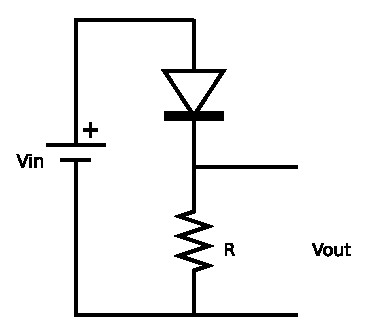
\includegraphics{Diagram1.eps}
\caption{Half wave rectifier.}\label{fig:Half_wave_rectifier}
\end{figure}
%
% Figure: Image1
%
\begin{figure}
\center
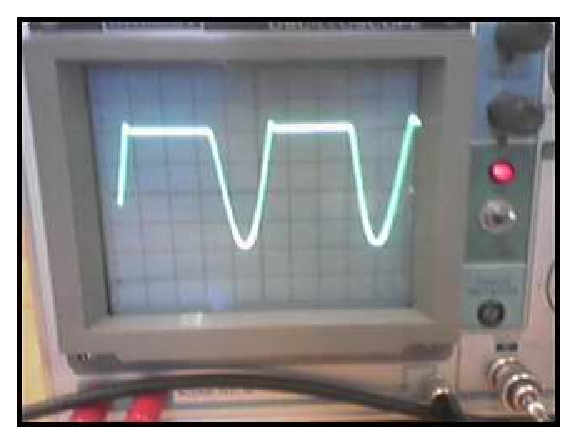
\includegraphics{Image1.eps} % See also dscn2393.jpg
\caption{$V_{out}$ as a function of time.}\label{fig:Image1} % Was fig:Q1
\end{figure}
%
% Figure: Image2
%
\begin{figure} % See also dscn2394.jpg & dscn2395.jpg
\center
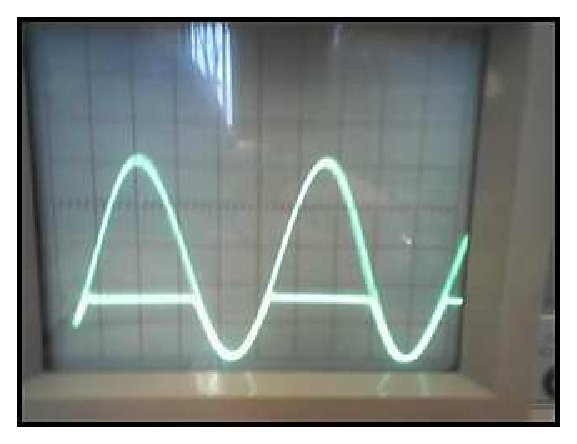
\includegraphics{Image2.eps}
\caption{$V_{out}$ related to $V_{in}$. $V_{in}$ is the full wave while $V_{out}$ is the trundacted wave.}\label{fig:Image2} % Was fig:Q1
\end{figure}

The full wave rectifier circuit shown in figure \ref{fig:Full_wave_rectifier} was assembled with $R = 20$ k$\Omega$ and using a TC016 symmetric transformer, which has equal impedances in both windings. This transformer also has a center tap which allows the rectifier to be made with only two diodes. Figure \ref{fig:Image3} shows $V_{out}$ compared with $V_{in}$, where  $V_{out}$ is truncated at voltages above -0.2 V\footnote{Answer to question 4.}.
%
% Figure: Diagram 2
%
\begin{figure}
\begin{center}
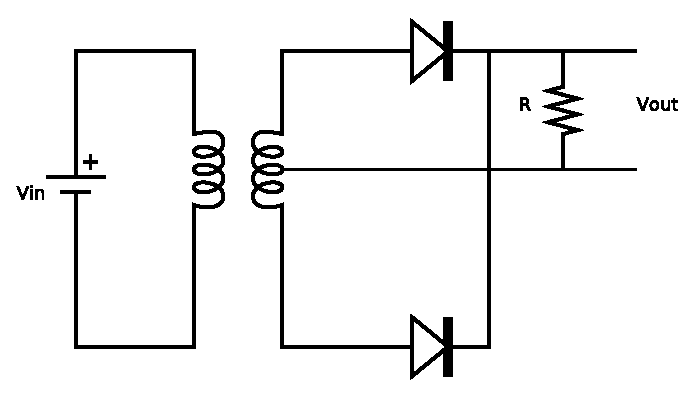
\includegraphics{Diagram2.eps}
\end{center}
\caption{Full wave rectifier.}\label{fig:Full_wave_rectifier}
\end{figure}
%
% Figure: Image 3
%
\begin{figure}
\begin{center}
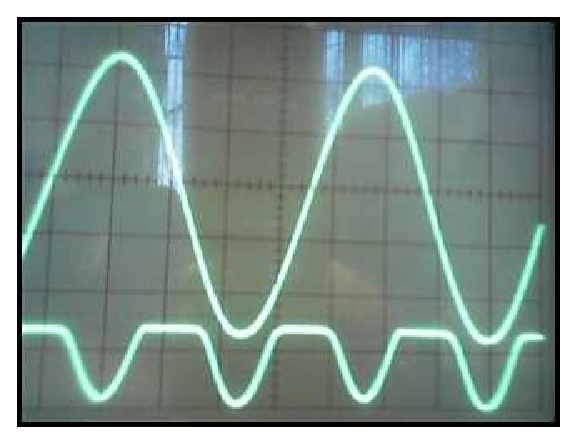
\includegraphics{Image3.eps}
\end{center}
\caption{Output.}\label{fig:Image3}
\end{figure}

A 5000 pF capacitor was then added in parallel with resistor $R$ and had no effect on the circuit\footnote{Answer to question 5.}. A much larger capacitor of 0.1 $\mu$F was inserted in place of the 5000 pF capacitor. Figure \ref{fig:Image4} and Figure \ref{fig:Image4} show the circuit output with no capacitor and with a 0.1 $\mu$F capacitor respectivly\footnote{Answer to question 6.}. To keep the voltage variation to less than 1\% at 996 Hz the capacitor would have to be approximatly 161 $\mu$F\footnote{Answer to question 7.}.
%
% Figure: Image 4
%
\begin{figure}
\begin{center}
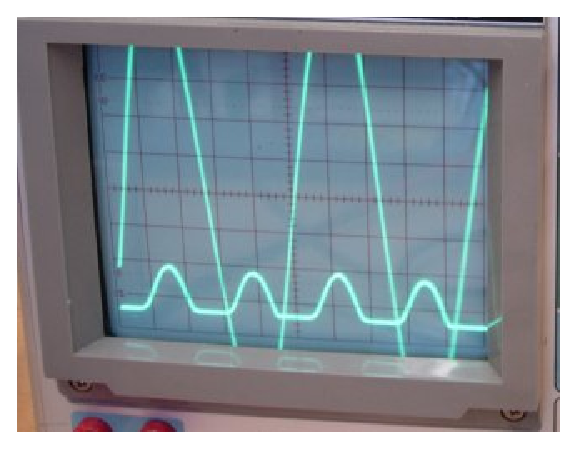
\includegraphics{Image4.eps}
\end{center}
\caption{Before.}\label{fig:Image4}
\end{figure}
%
% Figure: Image 4
%
\begin{figure}
\begin{center}
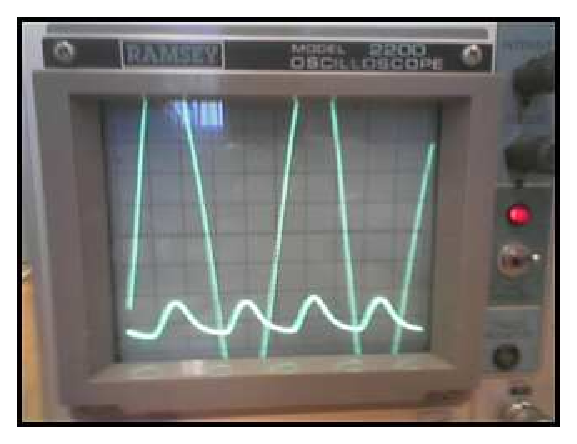
\includegraphics{Image5.eps}
\end{center}
\caption{After.}\label{fig:Image5}
\end{figure}

\subsection{Part B: Transistors}
Two simple circuits were constructed to investigate the nature and behavior of transistors. A two resistor voltaage divider with $R_1 = 912\ \Omega$ and $R_2 = 911\ \Omega$ and $V_{in} = 11.9$ V constructed. $V_{out}$ was measured to be $V_{out} = 5.99$ V\footnote{Answer to the first part of question 8.}. A load resistor of $R_{load} = 510\ \Omega$ was placed in parallel with $R_2$ and the output voltage was then measured to be $V_{out} = 3.05$ V. Figure \ref{fig:plot01} shows the relationship between the output voltage as a function of the output current across the load resistor. The output impedance of the voltage divider is given by sum of parallel resistors, Equation \ref{eq:resistor-parallel}.
\begin{equation}\label{eq:resistor-parallel}
Z = \frac{R_2 R_{load}}{R_2 + R_{load}}
\end{equation}
Which yields\footnote{Answer to question 9.}
\begin{displaymath}
Z = \frac{911\ \Omega\ 510\ \Omega}{911\ \Omega\ + 510\ \Omega} = 326\ \Omega
\end{displaymath}
%
% Figure: Plot01
%
\begin{figure}
\input{plot01}
\caption{This is the caption. It should include a short description of the figure.}\label{fig:plot01}
\end{figure}

The cicuit shown in figure \ref{fig:diagram3} was constructed the above voltage divider, sans $R_{load}$, using a 2N3904 NPN transistor and $R_e =1000\ \Omega$. The output voltage was measured as $V_{out} = 5.31$ V and the voltage across $R_e$ as... \footnote{Answer this question 10.}.
%
% Figure: Diagram3
%
\begin{figure}
\begin{center}
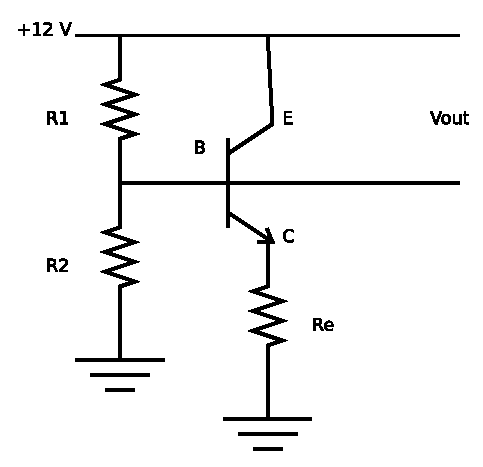
\includegraphics{Diagram3.eps}
\end{center}
\caption{Circuit diagram.}\label{fig:diagram3}
\end{figure}

A 510 $\Omega$ load resistor was added in parallel with $R_e$ and the output voltage measured as $V_{out} = 5.26$ V. The results are plotted in Figure \ref{fig:plot01} and compared to the voltage divider measurements\footnote{Answer to question 11.}.

%=========================%
%--> Sec: Bibliography <--%
%=========================%
%\begin{thebibliography}{9}
% This command tells LaTeX to create "References" section containing all the references that are not commented out. Be sure to uncomment all the references which you use and add those that are not currently listed.
%\%bibitem{Manual} Lab manual
%\end{thebibliography}

\end{document}

%=================%
%--> Templates <--%
%=================%
% This section contains templates for commonly used environments. This section will not appear in you final document as it come after the "\end{document}" command above.

% Equation template
\begin{equation}\label{eq:eqLabel}
math = good^2
\end{equation}

% Figure template
\begin{figure}
\input{graphicFile}
\caption{This is the caption. It should include a short description of the figure.}\label{fig:figureLabel}
\end{figure}
